%=============================================================================
%=============================================================================

\chapter{Semi-Structured-Grid System Interface (SStruct)}
\label{ch-SStruct}

The \code{SStruct} interface is appropriate for applications with grids that
are mostly---but not entirely---structured, e.g. block-structured grids (see
Figure~\ref{fig-sstruct-example}), composite grids in structured adaptive mesh
refinement (AMR) applications (see Figure~\ref{fig-sstruct-samr-grid}), and
overset grids.  In addition, it supports more general PDEs than the
\code{Struct} interface by allowing multiple variables (system PDEs) and
multiple variable types (e.g. cell-centered, face-centered, etc.).  The
interface provides access to data structures and linear solvers in \hypre{}
that are designed for semi-structured grid problems, but also to the most
general data structures and solvers.  These latter solvers are usually provided
via the \code{FEI} or \code{IJ} interfaces described in Chapters~\ref{ch-FEI}
and \ref{ch-IJ}.

The \code{SStruct} grid is composed out of a number of structured grid {\em
parts}, where the physical inter-relationship between the parts is arbitrary.
Each part is constructed out of two basic components: boxes (see
Figure~\ref{fig-struct-boxes}) and {\em variables}.  Variables represent the
actual unknown quantities in the grid, and are associated with the box indices
in a variety of ways, depending on their types.  In \hypre{}, variables may be
cell-centered, node-centered, face-centered, or edge-centered.  Face-centered
variables are split into x-face, y-face, and z-face, and edge-centered
variables are split into x-edge, y-edge, and z-edge.  See Figure
\ref{fig-gridvars} for an illustration in 2D.

\begin{figure}
\centering
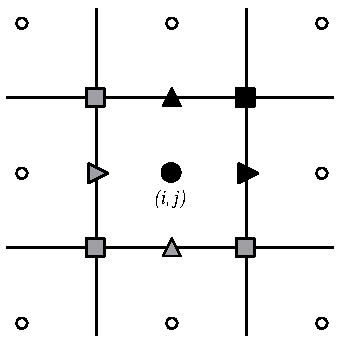
\includegraphics[width=.3\textwidth]{figSStructGridVars}
\caption{%
Grid variables in \hypre{} are referenced by the abstract cell-centered index
to the left and down in 2D (analogously in 3D).  In the figure, index $(i,j)$
is used to reference the variables in black.  The variables in grey---although
contained in the pictured cell---are not referenced by the $(i,j)$ index.}
\label{fig-gridvars}
\end{figure}

The \code{SStruct} interface uses a {\em graph} to allow nearly arbitrary
relationships between part data.  The graph is constructed from stencils plus
some additional data-coupling information set by the \code{GraphAddEntries()}
routine.  Another method for relating part data is the
\code{GridSetNeighborPart()} routine, which is particularly suited for
block-structured grid problems.

There are five basic steps involved in setting up the linear system to be
solved:
%\begin{enumerate}
\begin{list}{\arabic{enumi}.}{\usecounter{enumi}\setlength{\itemsep}{0in}}
\item set up the grid,
\item set up the stencils,
\item set up the graph,
\item set up the matrix,
\item set up the right-hand-side vector.
\end{list}
%\end{enumerate}

%-----------------------------------------------------------------------------

\section{Block-Structured Grids}
\label{sec-Block-Structured-Grids}

In this section, we describe how to use the \code{SStruct} interface to
define block-structured grid problems.  We will do this primarily by
example, paying particular attention to the construction of stencils
and the use of the \code{GridSetNeighborPart()} interface routine.

Consider the solution of the diffusion equation
\begin{equation} \label{eqn-block-diffusion}
- \nabla \cdot (D \nabla u) + \sigma u = f
\end{equation}
on the block-structured grid in Figure~\ref{fig-sstruct-example}, where $D$ is
a scalar diffusion coefficient, and $\sigma \geq 0$.  The discretization
\cite{JEMorel_RMRoberts_MJShashkov_1998} introduces three different types of
variables: cell-centered, $x$-face, and $y$-face.  The three discretization
stencils that couple these variables are also given in the figure.  The
information in this figure is essentially all that is needed to describe the
nonzero structure of the linear system we wish to solve.
\begin{figure}
\centering
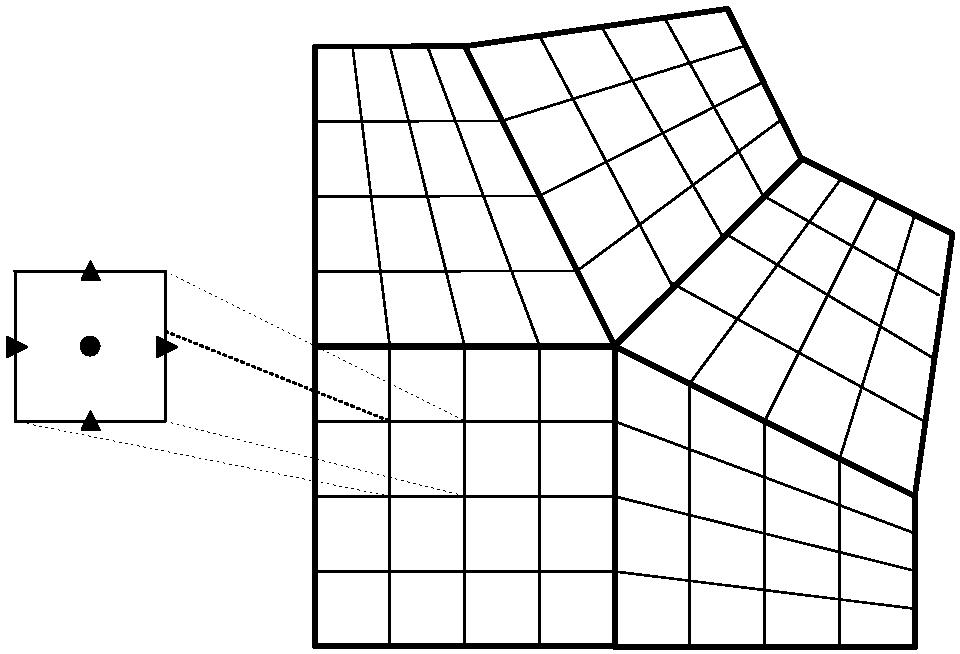
\includegraphics[width=.4\textwidth]{figSStructExample1a}
\hfill
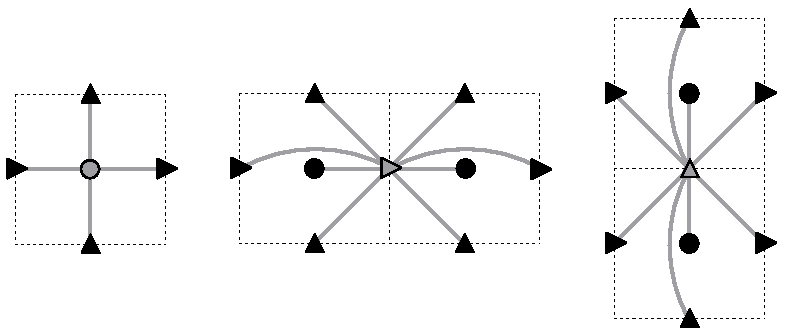
\includegraphics[width=.4\textwidth]{figSStructExample1b}
\caption{%
Example of a block-structured grid with five logically-rectangular blocks and
three variables types: cell-centered, $x$-face, and $y$-face.  Discretization
stencils for the cell-centered (left), $x$-face (middle), and $y$-face (right)
variables are also pictured.}
\label{fig-sstruct-example}
\end{figure}

The grid in Figure~\ref{fig-sstruct-example} is defined in terms of five
separate logically-rectangular parts as shown in
Figure~\ref{fig-sstruct-example-parts}, and each part is given a unique label
between 0 and 4.  Each part consists of a single box with lower index $(1,1)$
and upper index $(4,4)$ (see Section~\ref{sec-Struct-Grid}), and the grid data
is distributed on five processes such that data associated with part~$p$ lives
on process~$p$.  Note that in general, parts may be composed out of arbitrary
unions of boxes, and indices may consist of non-positive integers (see
Figure~\ref{fig-struct-boxes}).  Also note that the \code{SStruct} interface
expects a domain-based data distribution by boxes, but the actual distribution
is determined by the user and simply described (in parallel) through the
interface.

\begin{figure}
\centering
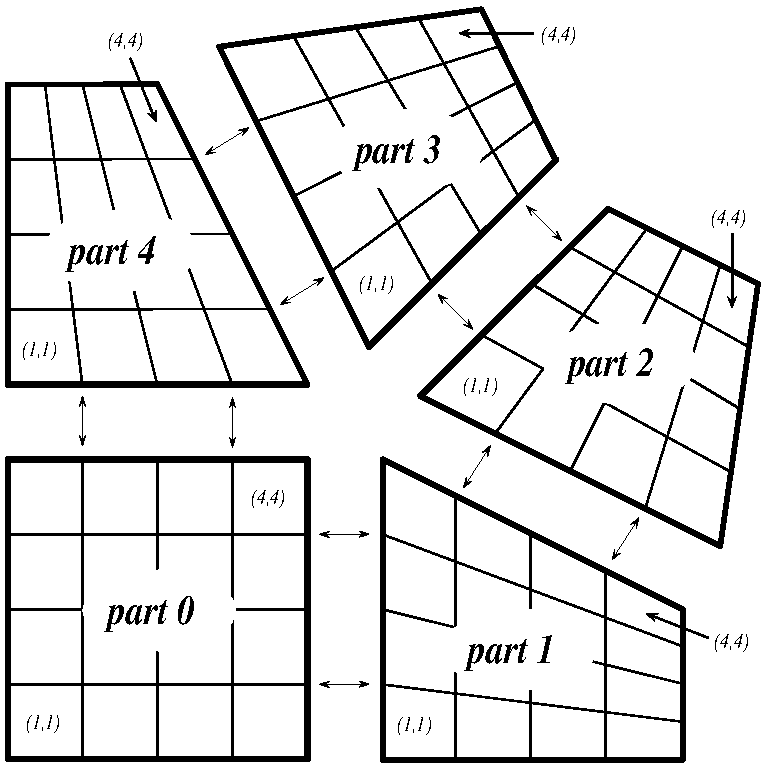
\includegraphics[width=.4\textwidth]{figSStructExample1c}
\caption{%
Test figure.}
\label{fig-sstruct-example-parts}
\end{figure}

As with the \code{Struct} interface, each process describes that portion of the
grid that it ``owns'', one box at a time.  Figure~\ref{fig-sstruct-grid} shows
the code for setting up the grid on process~3 (the code for the other processes
is similar).
\begin{figure}
\centering
\begin{tabular}{@{}c@{}}
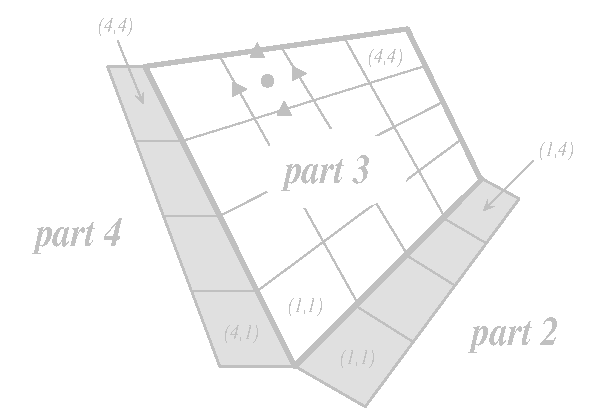
\includegraphics[width=.28\textwidth]{figSStructGrid1} \\ 1
\end{tabular}
\hfill
\begin{tabular}{@{}c@{}}
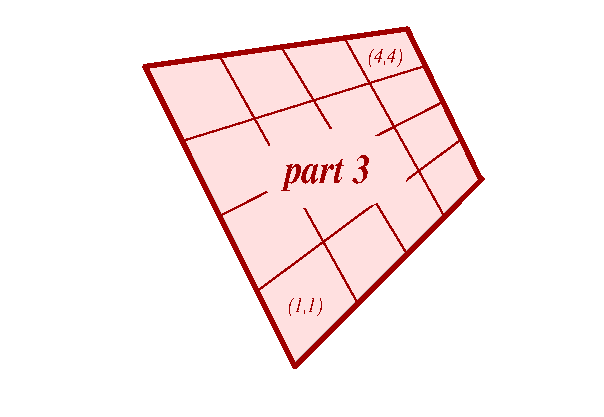
\includegraphics[width=.28\textwidth]{figSStructGrid2} \\ 2
\end{tabular}
\hfill
\begin{tabular}{@{}c@{}}
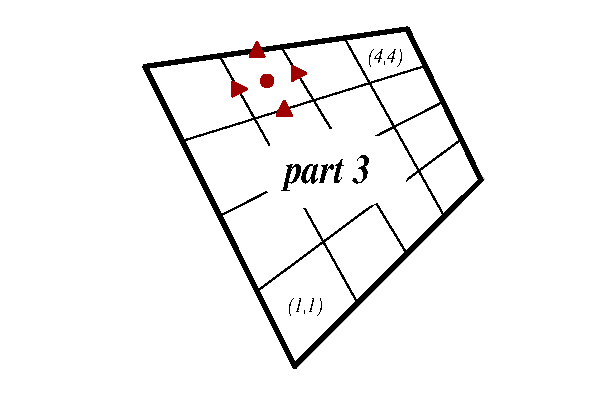
\includegraphics[width=.28\textwidth]{figSStructGrid3} \\ 3
\end{tabular}
\vspace{1em} \\
\begin{tabular}{@{}c@{}}
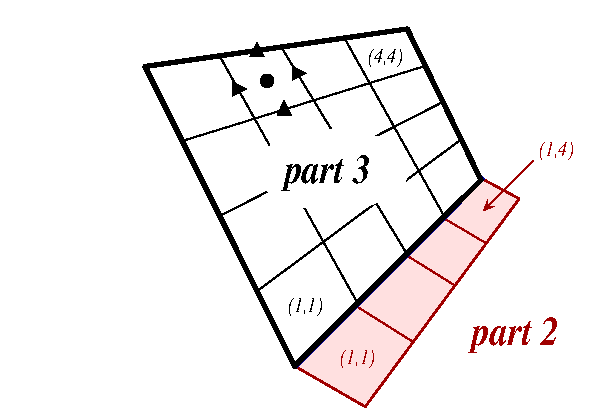
\includegraphics[width=.28\textwidth]{figSStructGrid4} \\ 4
\end{tabular}
\hfill
\begin{tabular}{@{}c@{}}
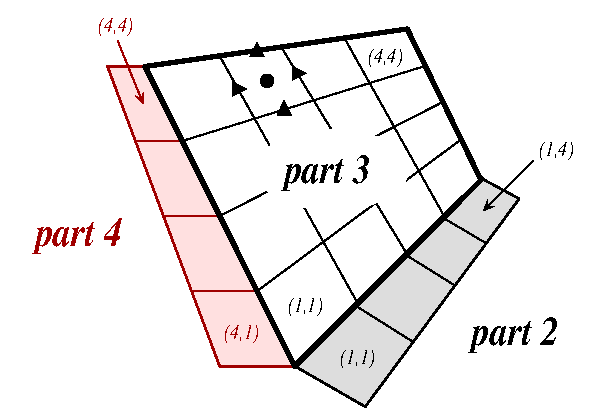
\includegraphics[width=.28\textwidth]{figSStructGrid5} \\ 5
\end{tabular}
\hfill
\begin{tabular}{@{}c@{}}
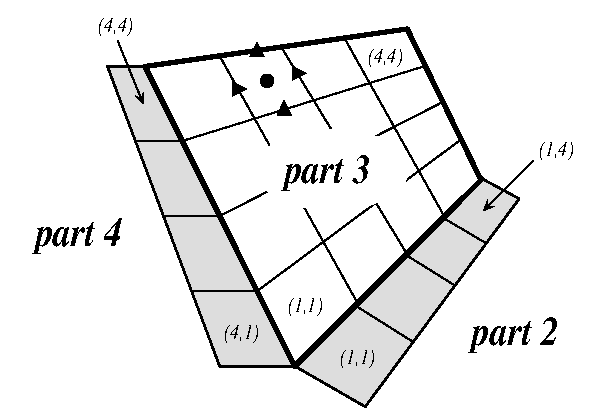
\includegraphics[width=.28\textwidth]{figSStructGrid6} \\ 6
\end{tabular}
\vspace{2em} \\
\begin{minipage}{0.9\textwidth}
\begin{verbatim}
    
    HYPRE_SStructGrid grid;
    int ndim = 2, nparts = 5, nvars = 3, part = 3;
    int extents[][2] = {{1,1}, {4,4}};
    int vartypes[]   = {HYPRE_SSTRUCT_VARIABLE_CELL,
                        HYPRE_SSTRUCT_VARIABLE_XFACE,
                        HYPRE_SSTRUCT_VARIABLE_YFACE};
    int nb2_n_part      = 2,              nb4_n_part      = 4;
    int nb2_exts[][2]   = {{1,0}, {4,0}}, nb4_exts[][2]   = {{0,1}, {0,4}};
    int nb2_n_exts[][2] = {{1,1}, {1,4}}, nb4_n_exts[][2] = {{4,1}, {4,4}};
    int nb2_map[2]      = {1,0},          nb4_map[2]      = {0,1};
    int nb2_dir[2]      = {1,-1},         nb4_dir[2]      = {1,1};

1:  HYPRE_SStructGridCreate(MPI_COMM_WORLD, ndim, nparts, &grid);
    
    /* Set grid extents and grid variables for part 3 */
2:  HYPRE_SStructGridSetExtents(grid, part, extents[0], extents[1]);
3:  HYPRE_SStructGridSetVariables(grid, part, nvars, vartypes);
    
    /* Set spatial relationship between parts 3 and 2, then parts 3 and 4 */
4:  HYPRE_SStructGridSetNeighborPart(grid, part, nb2_exts[0], nb2_exts[1],
       nb2_n_part, nb2_n_exts[0], nb2_n_exts[1], nb2_map, nb2_dir);
5:  HYPRE_SStructGridSetNeighborPart(grid, part, nb4_exts[0], nb4_exts[1],
       nb4_n_part, nb4_n_exts[0], nb4_n_exts[1], nb4_map, nb4_dir);
    
6:  HYPRE_SStructGridAssemble(grid);
    
\end{verbatim}
\end{minipage}
\caption{%
Code on process 3 for setting up the grid in Figure~\ref{fig-sstruct-example}.}
\label{fig-sstruct-grid}
\end{figure}
The ``icons'' at the top of the figure illustrate the result of the numbered
lines of code.  Process~3 needs to describe the data pictured in the
bottom-right of the figure.  That is, it needs to describe part~3 plus some
additional neighbor information that ties part~3 together with the rest of the
grid.  The \code{Create()} routine creates an empty 2D grid object with five
parts that lives on the \code{MPI_COMM_WORLD} communicator.  The
\code{SetExtents()} routine adds a new box to the grid.  The
\code{SetVariables()} routine associates three variables of type cell-centered,
$x$-face, and $y$-face with part~3.

At this stage, the description of the data on part~3 is complete.  However, the
spatial relationship between this data and the data on neighboring parts is not
yet defined.  To do this, we need to relate the index space for part~3 with the
index spaces of parts 2 and~4.  More specifically, we need to tell the interface
that the two grey boxes neighboring part~3 in the bottom-right of
Figure~\ref{fig-sstruct-grid} also correspond to boxes on parts 2 and~4.  This
is done through the two calls to the \code{SetNeighborPart()} routine.  We will
discuss only the first call, which describes the grey box on the right of the
figure.  Note that this grey box lives outside of the box extents for the grid
on part~3, but it can still be described using the index-space for part~3
(recall Figure~\ref{fig-struct-boxes}).  That is, the grey box has extents
$(1,0)$ and $(4,0)$ on part~3's index-space, which is outside of part~3's grid.
The arguments for the \code{SetNeighborPart()} call are simply the lower and
upper indices on part~3 and the corresponding indices on part~2.  The final two
arguments to the routine indicate that the positive $x$-direction on part~3
(i.e., the $i$ component of the tuple $(i,j)$) corresponds to the positive
$y$-direction on part~2 and that the positive $y$-direction on part~3
corresponds to the positive $x$-direction on part~2.

The \code{Assemble()} routine is a collective call (i.e., must be called on all
processes from a common synchronization point), and finalizes the grid
assembly, making the grid ``ready to use''.

With the neighbor information, it is now possible to determine where off-part
stencil entries couple.  Take, for example, any shared part boundary such as
the boundary between parts 2 and~3.  Along these boundaries, some stencil
entries reach outside of the part.  If no neighbor information is given, these
entries are effectively zeroed out, i.e., they don't participate in the
discretization.  However, with the additional neighbor information, when a
stencil entry reaches into a neighbor box it is then coupled to the part
described by that neighbor box information.

Another important consequence of the use of the \code{SetNeighborPart()} routine
is that it can declare variables on different parts as being the same.  For
example, the face variables on the boundary of parts 2 and~3 are recognized as
being shared by both parts (prior to the \code{SetNeighborPart()} call, there
were two distinct sets of variables).  Note also that these variables are of
different types on the two parts; on part~2 they are $x$-face variables, but on
part~3 they are $y$-face variables.

For brevity, we consider only the description of the $y$-face stencil in
Figure~\ref{fig-sstruct-example}, i.e. the third stencil in the figure.  To do
this, the stencil entries are assigned unique labels between 0 and 8 and their
``offsets'' are described relative to the ``center'' of the stencil.  This
process is illustrated in Figure \ref{fig-sstruct-stencil}.  Nine calls are
made to the routine \code{HYPRE_SStructStencilSetEntry()}.  As an example, the
call that describes stencil entry 5 in the figure is given the entry number~5,
the offset $(-1,0)$, and the identifier for the $x$-face variable (the variable
to which this entry couples).  Recall from Figure~\ref{fig-gridvars} the
convention used for referencing variables of different types.  The geometry
description uses the same convention, but with indices numbered relative to the
referencing index $(0,0)$ for the stencil's center.
Figure~\ref{fig-sstruct-graph} shows the code for setting up the graph .
\begin{figure}
\centering
\mbox{}\hfill
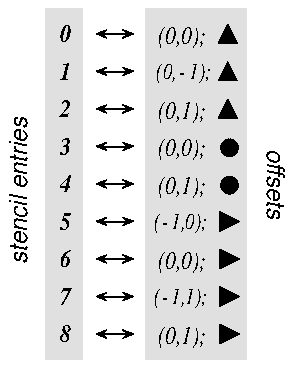
\includegraphics[width=.3\textwidth]{figSStructStenc0}
\hfill
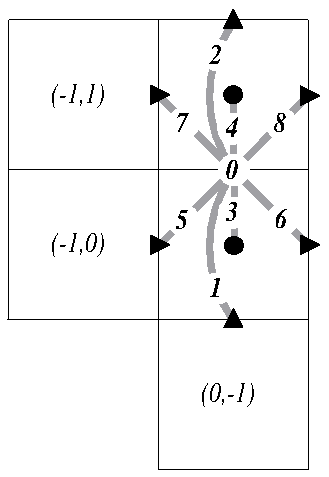
\includegraphics[width=.25\textwidth]{figSStructStenc1}
\hfill\mbox{}
\caption{%
Assignment of labels and geometries to the $y$-face stencil in
Figure~\ref{fig-sstruct-example}.  Stencil offsets are described relative to
the $(0,0)$ index for the ``center'' of the stencil.}
\label{fig-sstruct-stencil}
\end{figure}

\begin{figure}
\centering
\begin{tabular}{@{}c@{}}
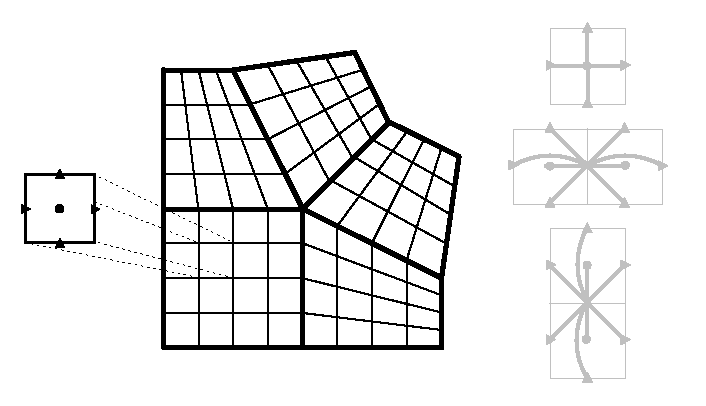
\includegraphics[width=.32\textwidth]{figSStructGraph1}\vspace{-.5em} \\ 1
\end{tabular}
\hfill
\begin{tabular}{@{}c@{}}
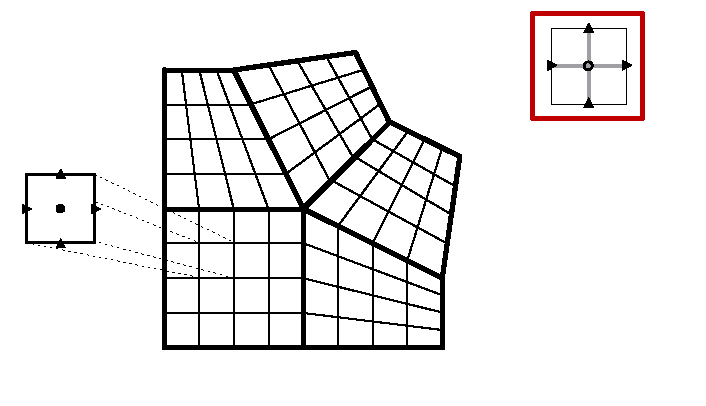
\includegraphics[width=.32\textwidth]{figSStructGraph2}\vspace{-.5em} \\ 2
\end{tabular}
\hfill
\begin{tabular}{@{}c@{}}
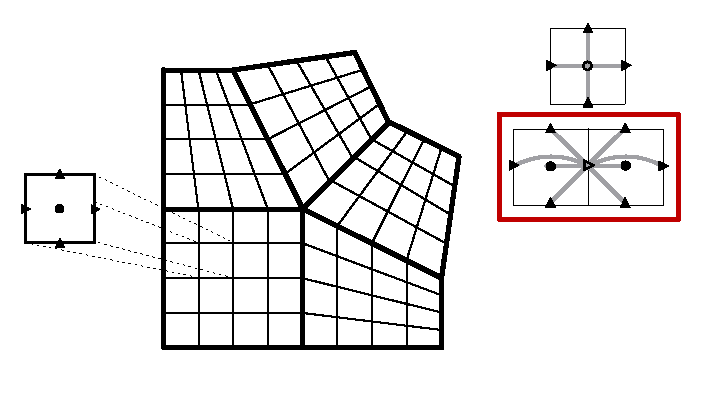
\includegraphics[width=.32\textwidth]{figSStructGraph3}\vspace{-.5em} \\ 3
\end{tabular}
\vspace{1em} \\
\mbox{}\hfill
\begin{tabular}{@{}c@{}}
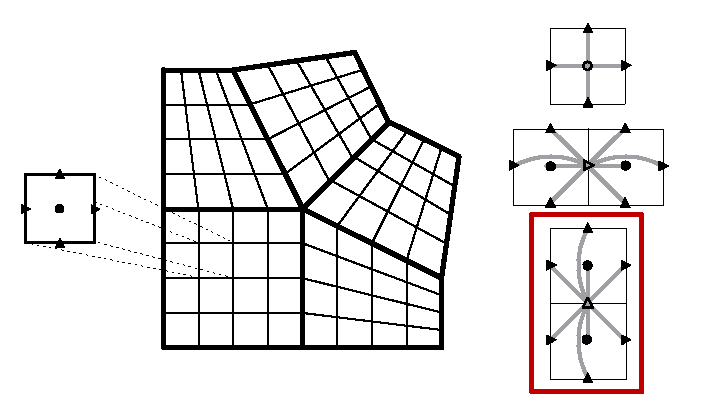
\includegraphics[width=.32\textwidth]{figSStructGraph4}\vspace{-.5em} \\ 4
\end{tabular}
\hfill
\begin{tabular}{@{}c@{}}
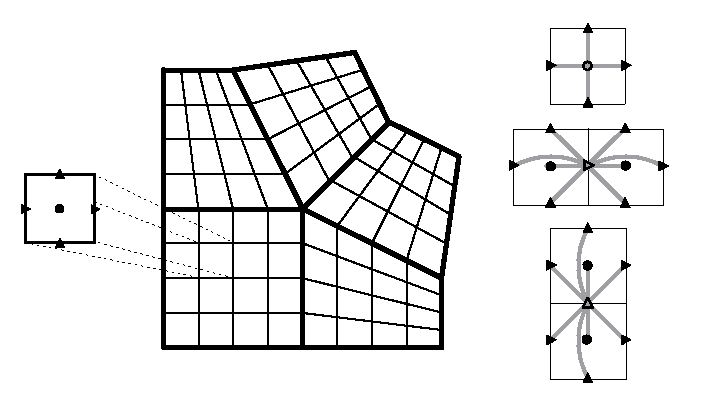
\includegraphics[width=.32\textwidth]{figSStructGraph5}\vspace{-.5em} \\ 5
\end{tabular}
\hfill\mbox{}
\vspace{2em} \\
\begin{minipage}{0.9\textwidth}
\begin{verbatim}
    
    HYPRE_SStructGraph graph;
    HYPRE_SStructStencil c_stencil, x_stencil, y_stencil;
    int c_var = 0, x_var = 1, y_var = 2;
    int part;
    
    /* Create the graph object */
1:  HYPRE_SStructGraphCreate(MPI_COMM_WORLD, grid, &graph);
    
    /* Set the cell-centered, x-face, and y-face stencils for each part */
    for (part = 0; part < 5; part++)
    {
2:     HYPRE_SStructGraphSetStencil(graph, part, c_var, c_stencil);
3:     HYPRE_SStructGraphSetStencil(graph, part, x_var, x_stencil);
4:     HYPRE_SStructGraphSetStencil(graph, part, y_var, y_stencil);
    }
    
    /* No need to add non-stencil entries in this example */
5:  HYPRE_SStructGraphAssemble(graph);

\end{verbatim}
\end{minipage}
\caption{%
Test figure.}
\label{fig-sstruct-graph}
\end{figure}

With the above, we now have a complete description of the nonzero structure for
the matrix.  The matrix coefficients are then easily set in a manner similar to
what is described in Section~\ref{sec-Struct-Matrix} using routines
\code{MatrixSetValues()} and \code{MatrixSetBoxValues()} in the \code{SStruct}
interface.  As before, there are also \code{AddTo} variants of these routines.
Likewise, setting up the right-hand-side is similar to what is described in
Section~\ref{sec-Struct-RHS}.  See the \hypre{} reference manual for details.

An alternative approach for describing the above problem through the interface
is to use the \code{GraphAddEntries()} routine instead of the
\code{GridSetNeighborPart()} routine.  In this approach, the five parts would be
explicitly ``sewn'' together by adding non-stencil couplings to the matrix
graph.  The main downside to this approach for block-structured grid problems
is that variables along block boundaries are no longer considered to be the
same variables on the corresponding parts that share these boundaries.  For
example, any face variable along the boundary between parts 2 and~3 in
Figure~\ref{fig-sstruct-example} would represent two different variables that
live on different parts.  To ``sew'' the parts together correctly, we would
need to explicitly select one of these variables as the representative that
participates in the discretization, and make the other variable a dummy
variable that is decoupled from the discretization by zeroing out appropriate
entries in the matrix.  All of these complications are avoided by using the
\code{GridSetNeighborPart()} for this example.

%-----------------------------------------------------------------------------

\section{Structured Adaptive Mesh Refinement}
\label{sec-Structured-Adaptive-Mesh-Refinement}

We now briefly discuss how to use the \code{SStruct} interface in a structured
AMR application.  Consider Poisson's equation on the simple cell-centered
example grid illustrated in Figure \ref{fig-sstruct-samr-grid}.  For structured
AMR applications, each refinement level should be defined as a unique part.
There are two parts in this example: part~0 is the global coarse grid and
part~1 is the single refinement patch.  Note that the coarse unknowns
underneath the refinement patch (gray dots in Figure
\ref{fig-sstruct-samr-grid}) are not real physical unknowns; the solution in
this region is given by the values on the refinement patch.  In setting up the
composite grid matrix \cite{SFMcCormick_1989a} for \hypre{} the equations for
these ``dummy'' unknowns should be uncoupled from the other unknowns (this can
easily be done by setting all off-diagonal couplings to zero in this region).

\begin{figure}
\centering
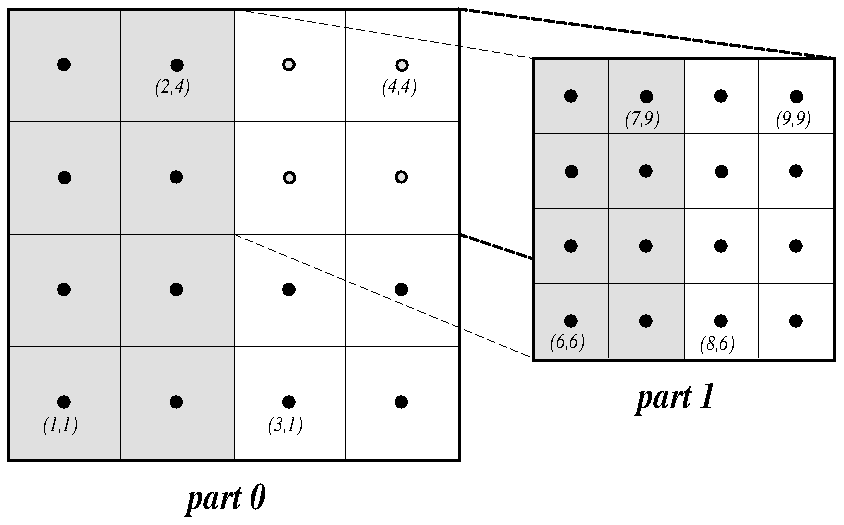
\includegraphics[width=.7\textwidth]{figSStructExample2a}
\caption{%
Structured AMR grid example. Shaded regions correspond to process~0, unshaded
to process~1.  The grey dots are dummy variables.}
\label{fig-sstruct-samr-grid}
\end{figure}

In the example, parts are distributed across the same two processes with
process 0 having the ``left'' half of both parts.  The composite grid is then
set up part-by-part by making calls to \code{GridSetExtents()} just as was done
in Section~\ref{sec-Block-Structured-Grids} and Figure~\ref{fig-sstruct-grid}
(no \code{SetNeighborPart} calls are made in this example).  Note that in the
interface there is no required rule relating the indexing on the refinement
patch to that on the global coarse grid; they are separate parts and thus each
has its own index space.  In this example, we have chosen the indexing such
that refinement cell $(2i,2j)$ lies in the lower left quadrant of coarse cell
$(i,j)$.  Then the stencil is set up.  In this example we are using a finite
volume approach resulting in the standard 5-point stencil in
Figure~\ref{fig-struct-stencil-b} in both parts.

The grid and stencil are used to define all intra-part coupling in the graph,
the non-zero pattern of the composite grid matrix.  The inter-part coupling at
the coarse-fine interface is described by \code{GraphAddEntries()} calls.  This
coupling in the composite grid matrix is typically the composition of an
interpolation rule and a discretization formula.  In this example, we use a
simple piecewise constant interpolation, i.e. the solution value in a coarse
cell is equal to the solution value at the cell center.  Then the flux across a
portion of the coarse-fine interface is approximated by a difference of the
solution values on each side.  As an example, consider approximating the flux
across the left interface of cell $(6,6)$ in Figure
\ref{fig-sstruct-samr-stencil}.  Let $h$ be the coarse grid mesh size, and
consider a local coordinate system with the origin at the center of cell
$(6,6)$.  We approximate the flux as follows
\begin{eqnarray}
\int_{-h/4}^{h/4}{u_x(-h/4,s)} ds
& \approx & \frac{h}{2} u_x(-h/4,0)
  \approx \frac{h}{2} \frac{u(0,0)-u(-3h/4,0)}{3h/4} \\
& \approx & \frac{2}{3} (u_{6,6}-u_{2,3}) \nonumber .
\end{eqnarray} 
The first approximation uses the midpoint rule for the edge integral, the second
uses a finite difference formula for the derivative, and the third the piecewise
constant interpolation to the solution in the coarse cell.  This means that the
equation for the variable at cell $(6,6)$ involves not only the stencil
couplings to $(6,7)$ and $(7,6)$ on part~1 but also non-stencil couplings to
$(2,3)$ and $(3,2)$ on part~0.  These non-stencil couplings are described by
\code{GraphAddEntries()} calls.  The syntax for this call is simply the part and
index for both the variable whose equation is being defined and the variable to
which it couples.  After these calls, the non-zero pattern of the matrix (and
the graph) is complete.  Note that the ``west'' and ``south'' stencil couplings
simply ``drop off'' the part, and are effectively zeroed out (currently, this is
only supported for the \code{HYPRE_PARCSR} object type, and these values must be
manually zeroed out for other object types; see \code{MatrixSetObjectType()} in
the reference manual).

\begin{figure}
\centering
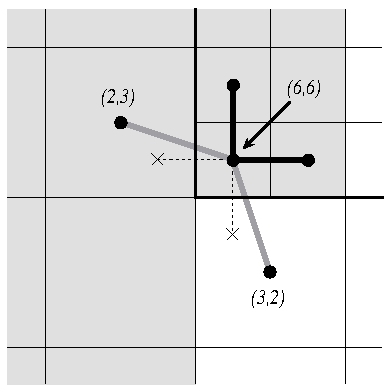
\includegraphics[width=.4\textwidth]{figSStructExample2b}
\caption{%
Coupling for equation at corner of refinement patch. Black lines
(solid and broken) are stencil couplings. Gray line are non-stencil
couplings.}
\label{fig-sstruct-samr-stencil}
\end{figure}

The remaining step is to define the actual numerical values for the composite
grid matrix.  This can be done by either \code{MatrixSetValues()} calls to set
entries in a single equation, or by \code{MatrixSetBoxValues()} calls to set
entries for a box of equations in a single call.  The syntax for the
\code{MatrixSetValues()} call is a part and index for the variable whose
equation is being set and an array of entry numbers identifying which entries
in that equation are being set.  The entry numbers may correspond to stencil
entries or non-stencil entries.
